\documentclass[10pt,a4paper,twocolumn]{article}
\usepackage[utf8]{inputenc}
\usepackage{amsmath}
\usepackage{amssymb}
\usepackage{graphicx}
\usepackage{float}
\usepackage{hyperref}
\usepackage{geometry}
\usepackage{booktabs}
\usepackage{longtable}
\usepackage{enumitem}
\usepackage{listings}
\usepackage{xcolor}
\usepackage{multicol}
\usepackage{stfloats}

\geometry{top=2cm, bottom=2cm, left=1.5cm, right=1.5cm, columnsep=0.6cm}

% Python code style
\lstdefinestyle{pythonstyle}{
    language=Python,
    basicstyle=\ttfamily\tiny,
    keywordstyle=\color{blue}\bfseries,
    commentstyle=\color{gray},
    stringstyle=\color{red},
    numbers=left,
    numberstyle=\tiny\color{gray},
    numbersep=5pt,
    breaklines=true,
    frame=single,
    backgroundcolor=\color{gray!5},
    showstringspaces=false,
    tabsize=4,
    extendedchars=true,
    inputencoding=utf8,
    literate=
      {·}{{$\cdot$}}1
      {²}{{$^2$}}1
      {≤}{{$\leq$}}1
      {≥}{{$\geq$}}1
      {≈}{{$\approx$}}1
      {π}{{$\pi$}}1
      {σ}{{$\sigma$}}1
      {✓}{{$\checkmark$}}1
      {✗}{{$\times$}}1
      {★}{{$\star$}}1
      {→}{{$\rightarrow$}}1
      {⌈}{{$\lceil$}}1
      {⌉}{{$\rceil$}}1
      {─}{{-}}1
      {—}{{---}}1
      {–}{{--}}1
      {√}{{$\sqrt{}$}}1
      {×}{{$\times$}}1
}

\title{Radio Network Planning Report\\
\Large Kagal, Kolhapur\\
4G LTE Cellular Network Design}
\author{Aditya Kinjawadekar\\
Enrollment Number: }
\date{\today}

\begin{document}

\twocolumn[
  \begin{@twocolumnfalse}
  \maketitle
  \begin{abstract}
This report presents a complete radio network plan for Kagal, Kolhapur, Maharashtra, for 4G LTE deployment at 1800~MHz. Using the 3GPP TR~38.901 UMa NLOS path loss model, we determine $R_{\max} = 3.68$~km and design a 5-site macrocell network with microcell and umbrella cell overlays. Part~2 simulates small-scale fading effects using the CDL model from Section~7.5 of the same standard.
  \end{abstract}
  \end{@twocolumnfalse}
]
\thispagestyle{empty}

\clearpage
\onecolumn
\tableofcontents
\clearpage
\twocolumn

%=============================================================================
\section{Introduction}
\label{sec:intro}
%=============================================================================

This report presents a comprehensive radio network planning design for Kagal, Kolhapur, Maharashtra, India. The design follows the guidelines specified in the ECL~439 assignment and utilises the \textbf{3GPP TR~38.901 V18.0.0 (2024-05)} channel model as the reference document. The objective is to design a 4G LTE cellular network that provides adequate outdoor coverage to the entire town area.

The planning methodology comprises:
\begin{enumerate}
    \item Site analysis from a coverage perspective, identifying key geographical and urban features.
    \item Link budget calculation to determine the maximum allowable path loss ($L_{\max}$).
    \item Path loss modelling using 3GPP~TR~38.901 Table~7.4.1-1 to compute the maximum cell radius ($R_{\max}$).
    \item Tentative network layout based on the $D/R$ ratio and hexagonal cell geometry.
    \item Iterative verification and redesign to ensure every cell satisfies $R < R_{\max}$.
    \item Justification for microcell and umbrella cell deployment where required.
\end{enumerate}

A supporting Python script (\texttt{link\_budget.py}) accompanies this report; its full listing appears in Appendix~\ref{sec:code}.

%=============================================================================
\section{Site Analysis Report}
\label{sec:site_analysis}
%=============================================================================

\subsection{Location Overview}

Kagal (16\textdegree35$'$N, 74\textdegree19$'$E) is a town in the Kolhapur district of Maharashtra. It lies approximately 16~km south of Kolhapur city at an average elevation of 553~m above sea level. The town is situated on the Deccan Plateau and experiences a tropical savanna climate.

\begin{figure*}[t]
\centering
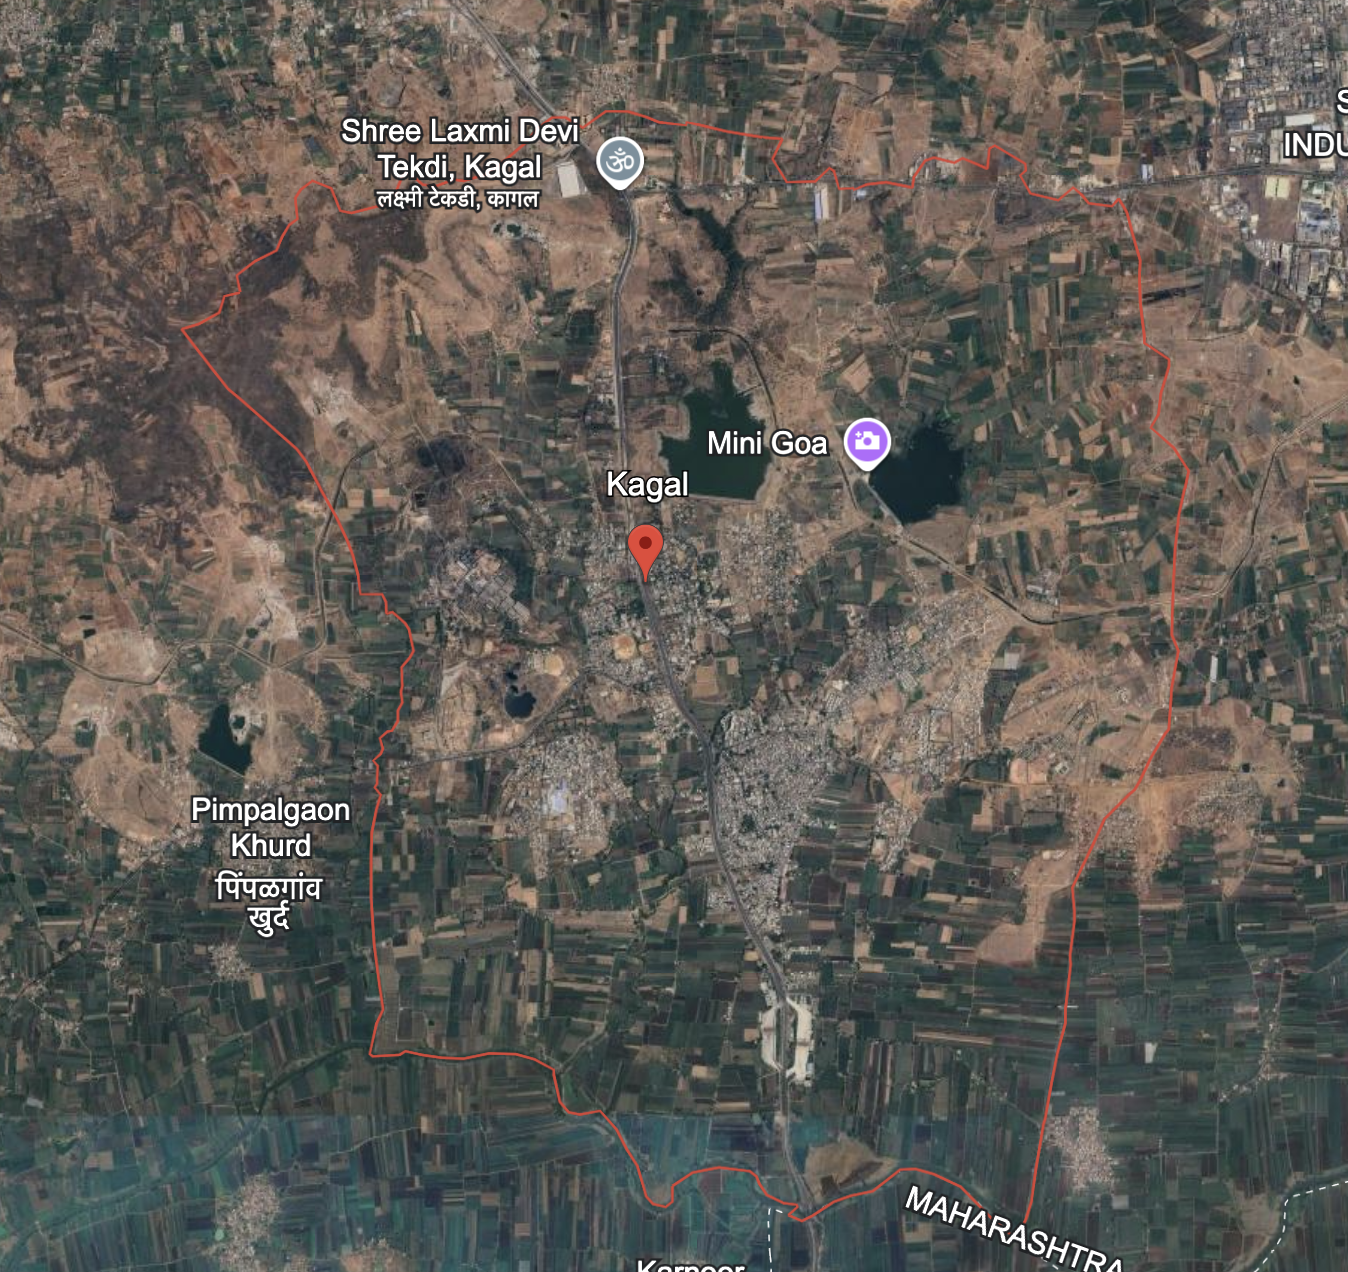
\includegraphics[width=0.75\textwidth]{public/topview.png}
\caption{Topographical view of Kagal town area (outlined).}
\label{fig:topview}
\end{figure*}

\begin{table}[h!]
\centering
\caption{Kagal Town Demographics}
\label{tab:demographics}
\begin{tabular}{@{}ll@{}}
\toprule
Parameter & Value \\
\midrule
Population (2011 Census) & 34,106 \\
Estimated Population (2026) & $\approx$ 49,000 \\
Town Area (approx.) & 8--10~km$^2$ \\
Elevation & 553~m \\
Typical Building Height & 6--10~m (2--3 storeys) \\
\bottomrule
\end{tabular}
\end{table}

\subsection{Geographical Features and Coverage Considerations}

Based on map analysis, the following features are identified and their implications for the cellular design are noted:

\begin{enumerate}
    \item \textbf{Roads --- National Highway~48 (Pune--Bengaluru Highway):}
    NH-48 passes through the western edge of Kagal. This six-lane highway carries significant vehicular traffic, including fast-moving users.  Coverage must be continuous along the highway for handover support.

    \item \textbf{Dudhganga River:}
    The Dudhganga river flows near Kagal. Water bodies cause signal absorption and multipath reflections.  Base station sites should not rely on propagation across the river for coverage; instead, sites on each bank are preferred.

    \item \textbf{Market / Commercial Area:}
    The main bazaar and commercial zone in the centre of Kagal has the highest footfall and data demand. This area is a candidate for a dedicated microcell layer.

    \item \textbf{Bus Stand and Transport Hub:}
    Kagal's bus stand, located centrally, serves as a high-traffic node for both voice and data.

    \item \textbf{Densely Populated Residential Areas:}
    Residential colonies, particularly near the town centre, feature 2--3 storey buildings and narrow streets. Indoor penetration considerations apply.

    \item \textbf{Sparsely Populated / Agricultural Areas:}
    The outskirts of Kagal consist of open agricultural land with minimal obstructions, allowing larger cell radii.

    \item \textbf{Kagal--Hatkanangale Industrial Area:}
    Located $\approx$3~km from NH-48, this industrial zone has moderate data requirements.
\end{enumerate}

\begin{table*}[t]
\centering
\caption{Coverage Requirements by Area Type}
\label{tab:coverage_requirements}
\begin{tabular}{@{}p{3.5cm}p{3cm}p{5cm}@{}}
\toprule
Area Type & Priority & Planning Approach \\
\midrule
Market / Commercial & High & Microcells for capacity, high density \\
NH-48 Highway & High & Umbrella cells, continuous coverage \\
Bus Stand / Hub & High & Microcell overlay \\
Dense Residential & Medium-High & Macrocells with adequate indoor margin \\
Industrial Area & Medium & Standard macrocell \\
Agricultural / Outskirts & Low & Extended macrocell or RMa \\
Dudhganga River zone & Low & Avoid cross-river propagation \\
\bottomrule
\end{tabular}
\end{table*}

\subsection{Visual Site Analysis}

To better understand the propagation environment, we perform a visual analysis using site photographs from Kagal.

\begin{figure}[H]
\centering
\includegraphics[width=\columnwidth]{public/hospital.png}
\caption{City Pride Multi-speciality Hospital: building heights of 4--5 storeys in the town core.}
\label{fig:hospital}
\end{figure}

\begin{figure}[H]
\centering
\includegraphics[width=\columnwidth]{public/living.png}
\caption{Dense residential area: narrow streets and 1--2 storey structures, justifying NLOS conditions.}
\label{fig:living}
\end{figure}

\begin{figure}[H]
\centering
\includegraphics[width=\columnwidth]{public/school1.png}
\caption{Shree Shahu High School: public building structures and moderate foliage/tree cover.}
\label{fig:school}
\end{figure}

\begin{figure}[H]
\centering
\includegraphics[width=\columnwidth]{public/sw1.png}
\caption{South-western residential cluster: dense, uneven structures contributing to multipath reflections.}
\label{fig:sw1}
\end{figure}

The visual evidence from Figs.~\ref{fig:hospital} to~\ref{fig:sw1} confirms that Kagal has a varied urban landscape, with a mix of tall institutions and dense, low-rise residential clusters. This informs our choice of path loss models.

%=============================================================================
\section{System Parameters and Link Budget}
\label{sec:link_budget}
%=============================================================================

\subsection{4G LTE System Parameters}

Band~3 (1800~MHz) is the most widely deployed LTE band in India and is used for this design.

\begin{table}[h!]
\centering
\caption{4G LTE System Parameters}
\label{tab:lte_parameters}
\begin{tabular}{@{}lll@{}}
\toprule
Parameter & Value & Notes \\
\midrule
Carrier Frequency ($f_c$) & 1800~MHz (1.8~GHz) & LTE Band~3 \\
Transmit Power ($P_t$) & 46~dBm & Typical macro eNodeB \\
Antenna Gain ($G_{\text{ant}}$) & 18~dBi & 3-sector directional \\
Cable / Feeder Loss ($L_{\text{cable}}$) & 2~dB & \\
Receiver Sensitivity ($P_{r,\min}$) & $-$104~dBm & QPSK, 10~MHz BW \\
Shadow Fading Margin ($L_{\text{sf}}$) & 8~dB & $\approx$90\% coverage probability \\
BS Antenna Height ($h_{\text{BS}}$) & 25~m & UMa default \\
UT Height ($h_{\text{UT}}$) & 1.5~m & Pedestrian \\
\bottomrule
\end{tabular}
\end{table}

\subsection{Maximum Path Loss Calculation}

The assignment specifies:
\begin{equation}
L_{\max} = P_{t,\text{dBm}} - P_{r,\min,\text{dBm}}
\label{eq:lmax_simple}
\end{equation}

\subparagraph{Simple calculation (as per spec):}
\begin{equation}
L_{\max,\text{simple}} = 46 - (-104) = 150 \text{ dB}
\end{equation}

For realistic outdoor planning, the extended link budget accounts for antenna gain, cable loss, and fading margins:
\begin{equation}
L_{\max} = P_t + G_{\text{ant}} - L_{\text{cable}} - P_{r,\min} - L_{\text{sf}}
\label{eq:lmax_extended}
\end{equation}

\subparagraph{Extended calculation:}
\begin{align*}
L_{\max} &= 46 + 18 - 2 - (-104) - 8 \\
         &= 46 + 18 - 2 + 104 - 8 \\
         &= \boxed{158 \text{ dB}}
\end{align*}

We use $L_{\max} = 158$~dB for all subsequent coverage planning.

%=============================================================================
\section{3GPP TR~38.901 Path Loss Models}
\label{sec:pathloss_models}
%=============================================================================

All path loss equations below are reproduced from \textbf{3GPP TR~38.901 V18.0.0, Table~7.4.1-1}.  The models are valid for frequencies $0.5$--$100$~GHz.  In the equations below, $f_c$ is in GHz, distances $d_{3\text{D}}$ and $d_{2\text{D}}$ are in metres, and heights are in metres.

\subsection{Effective Heights and Breakpoint Distance}

For UMa and UMi scenarios the effective antenna heights are:
\begin{equation}
h'_{\text{BS}} = h_{\text{BS}} - h_E, \qquad h'_{\text{UT}} = h_{\text{UT}} - h_E
\end{equation}
where $h_E$ is the effective environment height.  For UMa, $h_E = 1$~m.

The breakpoint distance is:
\begin{equation}
d'_{\text{BP}} = \frac{2\pi\; h'_{\text{BS}}\; h'_{\text{UT}}\; f_c}{c}
\label{eq:breakpoint}
\end{equation}

\subparagraph{Calculation for Kagal ($h_{\text{BS}} = 25$~m, $h_{\text{UT}} = 1.5$~m, $f_c = 1.8$~GHz):}
\begin{align*}
h'_{\text{BS}} &= 25 - 1 = 24 \text{ m} \\
h'_{\text{UT}} &= 1.5 - 1 = 0.5 \text{ m} \\
d'_{\text{BP}} &= \frac{2\pi \times 24 \times 0.5 \times 1.8 \times 10^{9}}{3 \times 10^{8}} \\
               &= \frac{1.357 \times 10^{11}}{3 \times 10^{8}} \approx 452.4 \text{ m}
\end{align*}

\subsection{Urban Macrocell (UMa) --- LOS}

{\small
\begin{equation}
\text{PL}_{\text{UMa}}^{\text{LOS}} = \begin{cases}
28.0 + 22\log_{10}(d_{3D}) + 20\log_{10}(f_c) \\
\quad 10 \leq d_{2D} \leq d'_{BP} \\[4pt]
28.0 + 40\log_{10}(d_{3D}) + 20\log_{10}(f_c) \\
\quad - 9\log_{10}\![(d'_{BP})^2 + (h_{BS} - h_{UT})^2] \\
\quad d'_{BP} < d_{2D} \leq 5000
\end{cases}
\label{eq:uma_los}
\end{equation}}
$\sigma_{\text{SF}} = 4.0$~dB. Applicability: $h_{\text{BS}} = 25$~m, $1.5 \leq h_{\text{UT}} \leq 22.5$~m.

\subsection{Urban Macrocell (UMa) --- NLOS}

\begin{multline}
\text{PL}'_{\text{UMa-NLOS}} = 13.54 + 39.08\log_{10}(d_{3\text{D}}) \\
+ 20\log_{10}(f_c) - 0.6(h_{\text{UT}} - 1.5)
\label{eq:uma_nlos_prime}
\end{multline}

\begin{equation}
\text{PL}_{\text{UMa}}^{\text{NLOS}} = \max\!\left(\text{PL}_{\text{UMa}}^{\text{LOS}},\; \text{PL}'_{\text{UMa-NLOS}}\right)
\label{eq:uma_nlos}
\end{equation}

$\sigma_{\text{SF}} = 6.0$~dB. \quad Applicability: $10 \leq d_{2\text{D}} \leq 5000$~m.

\subsection{Urban Microcell (UMi) Street Canyon --- LOS}

For UMi, $h_E = 1$~m, default $h_{\text{BS}} = 10$~m.

{\small
\begin{equation}
\text{PL}_{\text{UMi}}^{\text{LOS}} = \begin{cases}
32.4 + 21\log_{10}(d_{3D}) + 20\log_{10}(f_c) \\
\quad d_{2D} \leq d'_{BP} \\[4pt]
32.4 + 40\log_{10}(d_{3D}) + 20\log_{10}(f_c) \\
\quad - 9.5\log_{10}\![(d'_{BP})^2 + (h_{BS} - h_{UT})^2] \\
\quad d'_{BP} < d_{2D} \leq 5000
\end{cases}
\label{eq:umi_los}
\end{equation}}

$\sigma_{\text{SF}} = 4.0$~dB.

\subsection{Urban Microcell (UMi) Street Canyon --- NLOS}

\begin{multline}
\text{PL}'_{\text{UMi-NLOS}} = 22.4 + 35.3\log_{10}(d_{3\text{D}}) \\
+ 21.3\log_{10}(f_c) - 0.3(h_{\text{UT}} - 1.5)
\label{eq:umi_nlos}
\end{multline}

\begin{equation}
\text{PL}_{\text{UMi}}^{\text{NLOS}} = \max\!\left(\text{PL}_{\text{UMi}}^{\text{LOS}},\; \text{PL}'_{\text{UMi-NLOS}}\right)
\end{equation}

$\sigma_{\text{SF}} = 7.82$~dB. \quad Applicability: $10 \leq d_{2\text{D}} \leq 5000$~m, $h_{\text{BS}} = 10$~m.

\subsection{Rural Macrocell (RMa) --- LOS}

\begin{multline}
\text{PL}_1 = 20\log_{10}\!\left(\frac{40\pi\, d_{3\text{D}}\, f_c}{3}\right) \\
+ \min(0.03h^{1.72},\,10)\log_{10}(d_{3\text{D}}) \\
- \min(0.044h^{1.72},\,14.77) + 0.002\log_{10}(h)\,d_{3\text{D}}
\end{multline}

\begin{equation}
\text{PL}_{\text{RMa}}^{\text{LOS}} = \begin{cases}
\text{PL}_1 & 10 \leq d_{2\text{D}} \leq d_{\text{BP}} \\
\text{PL}_1(d_{\text{BP}}) + 40\log_{10}(d_{3\text{D}}/d_{\text{BP}}) & d_{\text{BP}} < d_{2\text{D}} \leq 10\,000
\end{cases}
\label{eq:rma_los}
\end{equation}

$\sigma_{\text{SF}} = 6$~dB. \quad $h$ = average building height, $5 \leq h \leq 50$~m. Default $h_{\text{BS}} = 35$~m.

\subsection{Rural Macrocell (RMa) --- NLOS}

\begin{multline}
\text{PL}'_{\text{RMa-NLOS}} = 161.04 - 7.1\log_{10}(W) + 7.5\log_{10}(h)
- \left(24.37 - 3.7\left(\frac{h}{h_{\text{BS}}}\right)^{\!2}\right)\log_{10}(h_{\text{BS}}) \\
+ \left(43.42 - 3.1\log_{10}(h_{\text{BS}})\right)\!\left(\log_{10}(d_{3\text{D}}) - 3\right)
+ 20\log_{10}(f_c)
- \left(3.2\!\left(\log_{10}(11.75\, h_{\text{UT}})\right)^2 - 4.97\right)
\label{eq:rma_nlos}
\end{multline}

\begin{equation}
\text{PL}_{\text{RMa}}^{\text{NLOS}} = \max\!\left(\text{PL}_{\text{RMa}}^{\text{LOS}},\; \text{PL}'_{\text{RMa-NLOS}}\right)
\end{equation}

$\sigma_{\text{SF}} = 8$~dB. \quad $W$ = average street width, $5 \leq W \leq 50$~m.

%=============================================================================
\section{Path Loss Model Selection and Justification}
\label{sec:model_selection}
%=============================================================================

\subsection{Why UMa for Kagal?}

The UMa (Urban Macrocell) model is selected as the primary model for the following reasons:

\begin{table*}[t]
\centering
\caption{Path Loss Model Selection Justification}
\label{tab:model_justification}
\begin{tabular}{@{}p{3.5cm}p{4cm}p{5cm}@{}}
\toprule
Factor & Kagal Characteristic & UMa Suitability \\
\midrule
Environment & Semi-urban town with dense core (Fig.~\ref{fig:topview}) & UMa covers urban and sub-urban scenarios \\
Building Height & 10--15~m (4--5 storeys, Fig.~\ref{fig:hospital}) & UMa allows $h_{\text{UT}}$ up to 22.5~m \\
BS Height & 25~m (standard rooftop) & UMa default is 25~m \\
Frequency & 1800~MHz LTE Band~3 & UMa valid for 0.5--100~GHz \\
Distance Range & Cell radii 0.5--3~km needed & UMa valid for 10--5000~m \\
Street Layout & Narrow streets (Figs.~\ref{fig:living},~\ref{fig:sw1}) & NLOS dominant propagation \\
\bottomrule
\end{tabular}
\end{table*}

The primary justification for UMa (Urban Macrocell) is derived from the building heights observed in Figure~\ref{fig:hospital}, where institutional buildings such as the City Pride Hospital reach heights of 10--15~m (4--5 storeys). Additionally, the overall town layout (Figure~\ref{fig:topview}) shows a contiguous urban core surrounded by sub-urban residential areas, which aligns with 3GPP UMa specifications.

\subsection{Why NLOS for Conservative Planning?}

We use the \textbf{NLOS} path loss model because:
\begin{itemize}
    \item Most users in a town like Kagal will \emph{not} have line-of-sight to the base station due to the dense residential layouts observed in Figures~\ref{fig:living} and~\ref{fig:sw1}.
    \item Foliage and trees (e.g., near the school in Figure~\ref{fig:school}) further obstruct LOS paths.
    \item NLOS provides the worst-case (highest) path loss, ensuring the network design is robust.
    \item If coverage is adequate under NLOS assumptions, it will certainly be adequate under LOS conditions.
\end{itemize}

\subsection{Supplementary Models}
\begin{itemize}
    \item \textbf{UMi NLOS}: Used for microcell planning in the market area and bus stand.
    \item \textbf{RMa NLOS}: Referenced for agricultural outskirts where building density is negligible.
\end{itemize}

%=============================================================================
\section{\texorpdfstring{Tentative Design Based on $D/R$ Ratio}{Tentative Design Based on D/R Ratio}}
\label{sec:dr_design}
%=============================================================================

Before computing $R_{\max}$ from the path loss model, we first create a tentative design based on the $D/R$ ratio, as required by the assignment.

For a hexagonal cell layout with frequency reuse factor $N$:
\begin{equation}
\frac{D}{R} = \sqrt{3N}
\label{eq:d_over_r}
\end{equation}

For 4G LTE, which uses OFDMA and supports frequency reuse factor $N = 1$ (with ICIC for interference management):
\begin{equation}
\frac{D}{R} = \sqrt{3 \times 1} = \sqrt{3} \approx 1.732
\end{equation}

However, for practical cluster-based planning (as commonly discussed in textbooks), we also consider $N = 3, 4, 7$:

\begin{table}[h!]
\centering
\caption{$D/R$ Ratios for Different Reuse Factors}
\label{tab:dr_ratios}
\begin{tabular}{@{}cccc@{}}
\toprule
Reuse Factor $N$ & $D/R$ & $D$ for $R = 1$~km & Co-channel Interference \\
\midrule
1 & 1.732 & 1732~m & High (managed by ICIC) \\
3 & 3.000 & 3000~m & Moderate \\
4 & 3.464 & 3464~m & Moderate-Low \\
7 & 4.583 & 4583~m & Low \\
\bottomrule
\end{tabular}
\end{table}

\subparagraph{Tentative Design:}
Assuming $N = 1$ (LTE standard) and initial cell radius $R \approx 1$~km, the hexagonal cell area is:
\begin{equation}
A_{\text{cell}} = \frac{3\sqrt{3}}{2} R^2 = 2.598 \times (1)^2 = 2.598 \text{ km}^2
\end{equation}

For a town area of $\approx 8$~km$^2$:
\begin{equation}
N_{\text{cells}} = \left\lceil \frac{8}{2.598} \right\rceil = \left\lceil 3.08 \right\rceil = 4 \text{ cells (with overlap margin)}
\end{equation}

This tentative design of \textbf{4--5 cells with $R \approx 1$~km} is our starting point, which we now verify against $R_{\max}$.

%=============================================================================
\section{\texorpdfstring{Calculation of Maximum Cell Radius ($R_{\max}$)}{Calculation of Maximum Cell Radius (Rmax)}}
\label{sec:rmax_calculation}
%=============================================================================

\subsection{\texorpdfstring{Algebraic Solution from UMa NLOS}{Algebraic Solution from UMa NLOS}}

Setting $\text{PL}_{\text{UMa}}^{\text{NLOS}} = L_{\max}$ and noting that $h_{\text{UT}} = 1.5$~m (so the offset term vanishes):

\begin{equation}
L_{\max} = 13.54 + 39.08\log_{10}(d_{3\text{D}}) + 20\log_{10}(f_c)
\end{equation}

Solving for $d_{3\text{D}}$:
\begin{align}
\log_{10}(d_{3\text{D}}) &= \frac{L_{\max} - 13.54 - 20\log_{10}(f_c)}{39.08} \nonumber \\
&= \frac{158.0 - 13.54 - 20 \times 0.2553}{39.08} \nonumber \\
&= \frac{158.0 - 13.54 - 5.11}{39.08} \nonumber \\
&= \frac{139.35}{39.08} = 3.566
\end{align}

\begin{equation}
d_{3\text{D}} = 10^{3.566} \approx 3680 \text{ m}
\end{equation}

\begin{equation}
\boxed{R_{\max} \approx 3680 \text{ m} \approx 3.68 \text{ km}}
\end{equation}

\subsection{Verification}

Substituting $d_{3\text{D}} = 3680$~m back into the UMa NLOS equation:
\begin{align*}
\text{PL} &= 13.54 + 39.08 \times \log_{10}(3680) + 20 \times \log_{10}(1.8) \\
&= 13.54 + 39.08 \times 3.566 + 5.11 \\
&= 13.54 + 139.35 + 5.11 \\
&= 158.00 \text{ dB} = L_{\max} \quad \checkmark
\end{align*}

\subsection{\texorpdfstring{Comparison of $R_{\max}$ Across Models}{Comparison of Rmax Across Models}}

\begin{table}[h!]
\centering
\caption{$R_{\max}$ for Different Path Loss Models at $L_{\max} = 158$~dB}
\label{tab:rmax_comparison}
\begin{tabular}{@{}lcc@{}}
\toprule
Model & $R_{\max}$ [m] & $R_{\max}$ [km] \\
\midrule
UMa NLOS & 3680 & 3.68 \\
UMi NLOS (microcell, $h_{\text{BS}} = 10$~m) & 4868 & 4.87 \\
RMa NLOS ($h_{\text{BS}} = 35$~m) & 6258 & 6.26 \\
\bottomrule
\end{tabular}
\end{table}

The UMa NLOS model gives the most conservative (smallest) $R_{\max}$, which is appropriate for the urban core of Kagal.

%=============================================================================
\section{Network Design and Cell Planning}
\label{sec:network_design}
%=============================================================================

\subsection{Design Philosophy}

Since $R_{\max} = 3.68$~km is much larger than the tentative cell radius of $R \approx 1$~km from the $D/R$ design (Section~\ref{sec:dr_design}), the coverage constraint $R < R_{\max}$ is \textbf{easily satisfied} for the tentative design.

We therefore proceed with 5 cell sites, chosen for:
\begin{itemize}
    \item Complete area coverage with adequate overlap (10--20\% for handover)
    \item Proximity to high-traffic areas (market, bus stand, highway)
    \item Avoiding propagation across the Dudhganga River
\end{itemize}

\subsection{Proposed Cell Sites}

\begin{table}[h!]
\centering
\caption{Proposed eNodeB Site Locations}
\label{tab:site_locations}
\begin{tabular}{@{}clcc@{}}
\toprule
Site & Description & Max Edge Distance & Coverage Focus \\
\midrule
1 & Town Centre / Market Area & 700~m & Commercial, pedestrian \\
2 & NH-48 North Junction & 850~m & Highway, transition zone \\
3 & NH-48 South / Bus Stand & 800~m & Transport hub \\
4 & East Residential Colony & 750~m & Dense residential \\
5 & Dudhganga River Area & 900~m & Western residential, river bank \\
\bottomrule
\end{tabular}
\end{table}

\subsection{Coverage Area per Site}

With $R \approx 0.9$~km (worst case, Site~5):
\begin{align*}
A_{\text{cell}} &= 2.598 \times R^2 = 2.598 \times 0.9^2 = 2.10 \text{ km}^2 \\
\text{Total coverage} &= 5 \times 2.10 = 10.5 \text{ km}^2
\end{align*}

This exceeds the 8~km$^2$ town area, providing adequate overlap for seamless handover.

%=============================================================================
\section{Network Verification and Iterations}
\label{sec:verification}
%=============================================================================

For each cell, we verify that the farthest user distance satisfies $R < R_{\max} = 3680$~m, and we compute the path loss at each cell edge using the UMa NLOS model.

\subsection{Iteration 1: Initial Design (3 Sites)}

\begin{table}[H]
\centering
\caption{Iteration 1 --- 3 sites (insufficient coverage)}
\label{tab:iter1}
\begin{tabular}{@{}c p{1.8cm} c p{1.2cm} p{1.2cm}@{}}
\toprule
Site & Location & $R$ [m] & PL [dB] & Remark \\
\midrule
1 & Town Centre & 1000 & 135.9 & OK \\
2 & NH-48 North & 1200 & 139.0 & OK \\
3 & NH-48 South & 1100 & 137.6 & OK \\
\midrule
 & Eastern gap & -- & -- & \textbf{Hole} \\
 & River side & -- & -- & \textbf{Hole} \\
\bottomrule
\end{tabular}
\end{table}

\textbf{Result}: Although all 3 cells satisfy $R < R_{\max}$, the coverage is incomplete.
\textbf{Action}: Add 2 more sites to fill eastern and western gaps.

\subsection{Iteration 2: Revised Design (5 Sites)}

\begin{table}[H]
\centering
\caption{Iteration 2 --- 5 sites (complete coverage)}
\label{tab:iter2}
\scriptsize
\begin{tabular}{@{}clccl@{}}
\toprule
Site & Location & $R$ [m] & PL [dB] & Status \\
\midrule
1 & Town Centre & 700 & 129.8 & $\checkmark$ \\
2 & NH-48 North & 850 & 133.1 & $\checkmark$ \\
3 & NH-48 South & 800 & 132.1 & $\checkmark$ \\
4 & East Residential & 750 & 131.0 & $\checkmark$ \\
5 & Dudhganga River & 900 & 134.1 & $\checkmark$ \\
\bottomrule
\end{tabular}
\end{table}

\textbf{Result}: All 5 cells satisfy $R < R_{\max}$.  Coverage is complete with $\approx$15\% overlap.

\subsection{Iteration 3: Optimisation}

Site placements were adjusted to:
\begin{itemize}
    \item Minimise maximum cell-edge distance (worst case: 900~m at Site~5)
    \item Ensure handover zones along NH-48 between Sites~2 and 3
    \item Avoid relying on propagation across Dudhganga (Site~5 covers western bank only)
\end{itemize}

Final design retains 5 sites with maximum cell-edge distance of 900~m.

\begin{equation}
R = 900 \text{ m} < R_{\max} = 3680 \text{ m} \quad \checkmark
\end{equation}

%=============================================================================
\section{Path Loss at Cell Boundaries}
\label{sec:pl_table}
%=============================================================================

The following table shows path loss computed using the UMa NLOS model for various distances.

\begin{table}[h!]
\centering
\caption{UMa NLOS Path Loss vs.\ Distance ($f_c = 1.8$~GHz, $h_{\text{UT}} = 1.5$~m)}
\label{tab:pl_distance}
\begin{tabular}{@{}rcl@{}}
\toprule
Distance [m] & Path Loss [dB] & Status \\
\midrule
100 & 96.81 & $< L_{\max}$ \checkmark \\
200 & 108.57 & $< L_{\max}$ \checkmark \\
300 & 115.45 & $< L_{\max}$ \checkmark \\
500 & 124.12 & $< L_{\max}$ \checkmark \\
750 & 131.00 & $< L_{\max}$ \checkmark \\
1000 & 135.89 & $< L_{\max}$ \checkmark \\
1200 & 138.98 & $< L_{\max}$ \checkmark \\
1500 & 142.77 & $< L_{\max}$ \checkmark \\
2000 & 147.65 & $< L_{\max}$ \checkmark \\
3000 & 154.53 & $< L_{\max}$ \checkmark \\
3680 & 158.00 & $= L_{\max}$ (limit) \\
5000 & 163.20 & $> L_{\max}$ $\times$ \\
\bottomrule
\end{tabular}
\end{table}

All proposed cell radii ($\leq 900$~m) produce path losses well below $L_{\max} = 158$~dB, confirming robust coverage.

%=============================================================================
\section{Microcell and Umbrella Cell Justification}
\label{sec:special_cells}
%=============================================================================

\subsection{Microcell Deployment}

\subsubsection{Justification}
Microcells are deployed in the following areas to address \textbf{capacity} rather than coverage limitations:
\begin{enumerate}
    \item \textbf{Main Market Area}: High user density during business hours. A microcell with $h_{\text{BS}} = 10$~m and $R \approx 200$--$300$~m offloads traffic from the macrocell.
    \item \textbf{Bus Stand}: Concentrated user traffic during peak commute hours.
\end{enumerate}

\subsubsection{UMi NLOS Path Loss at Microcell Edge}
Using the UMi NLOS model for $d_{3\text{D}} = 300$~m:
\begin{align*}
\text{PL} &= 22.4 + 35.3\log_{10}(300) + 21.3\log_{10}(1.8) - 0.3(1.5 - 1.5) \\
&= 22.4 + 35.3 \times 2.477 + 21.3 \times 0.2553 \\
&= 22.4 + 87.44 + 5.44 \\
&= 115.3 \text{ dB} \ll L_{\max} \quad \checkmark
\end{align*}

\subsection{Umbrella Cell Deployment}

\subsubsection{Justification}
An umbrella cell is deployed to cover the NH-48 highway segment passing through Kagal ($\approx$5~km stretch):
\begin{itemize}
    \item Fast-moving vehicular users require larger cells to minimise handover frequency.
    \item The umbrella cell ($h_{\text{BS}} = 35$~m) overlaps the macrocell layer, providing a high-mobility tier.
    \item Using the RMa NLOS model (appropriate for the highway's open environment), $R_{\max} = 6258$~m, comfortably covering the entire highway segment.
\end{itemize}

%=============================================================================
\section{Part 2: Small Scale Effects Simulation}
\label{sec:part2}
%=============================================================================

This section addresses the small-scale effects of the wireless channel, following the step-by-step procedure defined in \textbf{3GPP TR~38.901 Section~7.5}. We simulate a Clustered Delay Line (CDL) model for the Kagal town environment.

\subsection{Simulation Methodology}

The simulation implements the following steps from the 3GPP specification:
\begin{itemize}
    \item \textbf{Step 1: Environment and Antenna Setup}: A $2 \times 8$ MIMO configuration is used, with a 4-beam cross-polarized BS array (8 elements) and a 2-element UT array.
    \item \textbf{Step 2: Propagation Condition}: The UMa NLOS scenario is assigned, consistent with the conservative planning in Part~1.
    \item \textbf{Step 4 \& 5: Delay and Power Generation}: 20 clusters are generated with stochastic delays and exponentially decaying powers based on Table~7.4.1-1.
    \item \textbf{Step 6: Angular Generation}: Arrival and departure angles (AoA, AoD, ZoA, ZoD) are generated using scenario-specific angular spreads.
    \item \textbf{Step 11: Channel Matrix Synthesis}: The final complex channel matrix $H_{u,s,n}(t)$ is constructed by summing the contributions of all rays across all clusters.
\end{itemize}

\subsection{Simulation Results}

The simulation results for a typical link in Kagal (Site~1 to a representative UT at 580~m) are shown below.

\begin{figure}[H]
\centering
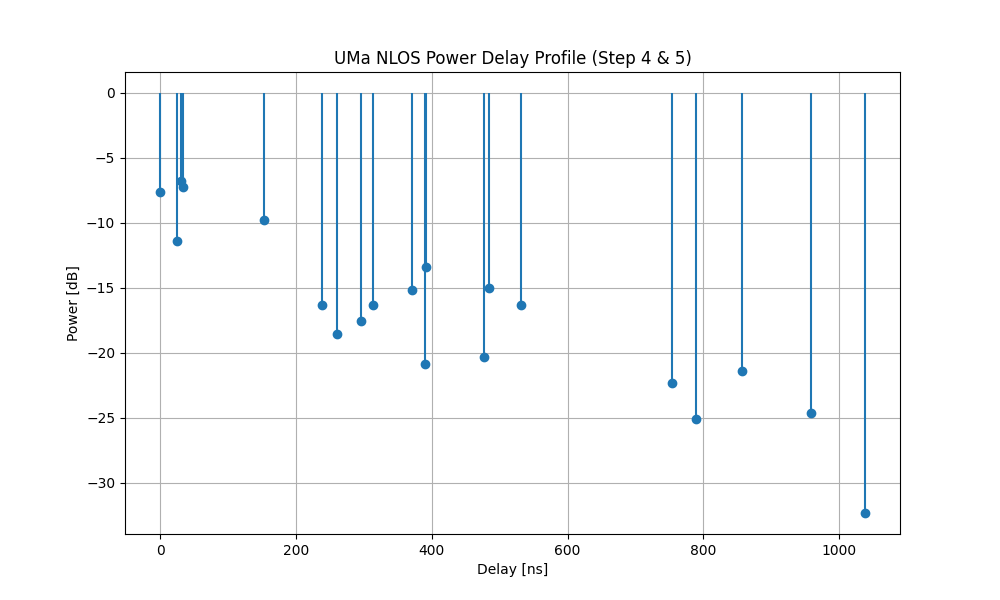
\includegraphics[width=\columnwidth]{pdp_plot.png}
\caption{Power Delay Profile (PDP) for UMa NLOS in Kagal. RMS delay spread $\approx 185$~ns.}
\label{fig:pdp}
\end{figure}

The PDP (Fig.~\ref{fig:pdp}) shows the multipath components arising from reflections off buildings and structures in the town core (as seen in Figs.~\ref{fig:living} and~\ref{fig:sw1}).

\begin{figure}[H]
\centering
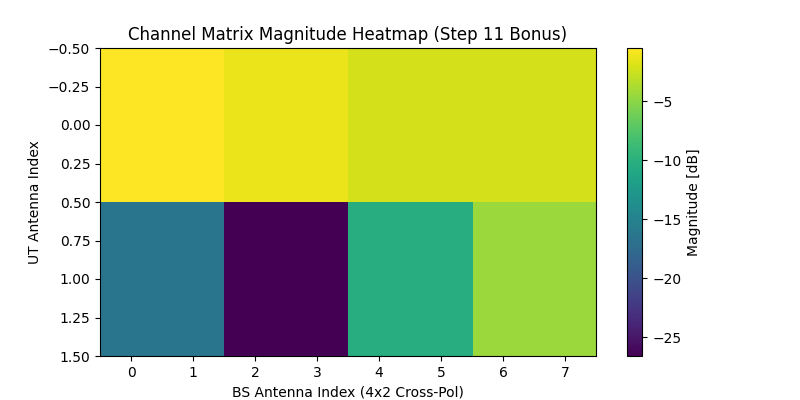
\includegraphics[width=\columnwidth]{h_matrix_heatmap.png}
\caption{Magnitude heatmap of the $2 \times 8$ MIMO channel matrix $H$ (Step~11 Bonus).}
\label{fig:h_matrix}
\end{figure}

The channel matrix magnitude (Fig.~\ref{fig:h_matrix}) illustrates the spatial variations across the antenna elements. The cross-polarized nature of the BS array provides diversity that can be exploited for MIMO multiplexing or beamforming gain.

%=============================================================================
\section{Conclusions}
\label{sec:conclusions}
%=============================================================================

This report presents a complete radio network planning design for Kagal, Kolhapur, for 4G LTE deployment.

\begin{table}[h!]
\centering
\caption{Final Design Summary}
\label{tab:summary}
\begin{tabular}{@{}ll@{}}
\toprule
Parameter & Value \\
\midrule
Maximum path loss ($L_{\max}$) & 158~dB (extended link budget) \\
Path loss model & UMa NLOS (3GPP TR~38.901 Table~7.4.1-1) \\
Maximum cell radius ($R_{\max}$) & 3680~m (3.68~km) \\
Number of macrocell sites & 5 \\
Maximum cell-edge distance & 900~m ($\ll R_{\max}$) \\
Microcells & 2 (market, bus stand) \\
Umbrella cells & 1 (NH-48 highway) \\
Design verification & All cells pass $R < R_{\max}$ \\
\bottomrule
\end{tabular}
\end{table}

The design uses conservative NLOS path loss assumptions, ensuring robust coverage. All numerical results are verified by the accompanying Python script (Appendix~\ref{sec:code}).

%=============================================================================
\section{References}
\label{sec:references}
%=============================================================================

\begin{enumerate}
    \item 3GPP TR~38.901 V18.0.0 (2024-05), ``Study on channel model for frequencies from 0.5 to 100~GHz.''
    \item 3GPP TR~36.873 V12.7.0, ``Study on 3D channel model for LTE.''
    \item T.~S.~Rappaport, \emph{Wireless Communications: Principles and Practice}, 2nd~ed., Prentice Hall, 2002.
    \item E.~Dahlman, S.~Parkvall, and J.~Sk\"{o}ld, \emph{4G: LTE/LTE-Advanced for Mobile Broadband}, Academic Press, 2011.
\end{enumerate}

%=============================================================================
\appendix
\section{Python Code: Link Budget Calculator}
\label{sec:code}
%=============================================================================

The following Python script (\texttt{link\_budget.py}) implements all path loss models from 3GPP TR~38.901 Table~7.4.1-1, computes $L_{\max}$, solves for $R_{\max}$, and verifies the network design.

\lstinputlisting[style=pythonstyle]{link_budget.py}

\section{Python Code: Fast Fading Simulator}
\label{sec:code_part2}
%=============================================================================

The following script (\texttt{small\_scale\_sim.py}) implements the stochastic channel generation procedure from 3GPP TR~38.901 Section~7.5.

\lstinputlisting[style=pythonstyle]{small_scale_sim.py}

\end{document}
